\pdfminorversion=4
\documentclass[aspectratio=169]{beamer}
\usepackage{animate} % for animation
\usepackage{array,multirow,graphicx}
\usepackage{multicol}
\usepackage{etoolbox}
\graphicspath{{/home/fafaa/Documents/sinyal_dan_sistem/Slide/gambar}}
\setbeamertemplate{caption}[numbered]
\setbeamertemplate{section in toc}[sections numbered]

% Hide subsubsections from TOC, but keep PDF bookmarks with beamer
\hypersetup{bookmarksopen=true,bookmarksopenlevel=4}
\setcounter{tocdepth}{4}

\renewcommand{\figurename}{Gambar.}
\renewcommand{\tablename}{Tabel.}

\usetheme[pageofpages=of,	% String used between the current page and the
							% total page count.
			alternativetitlepage=true,% Use the fancy title page.
			titleline=true,
			titlepagelogo=OK-LOGO-ITK.jpg
%          	 titlepagelogo=fig/jaist_logo.png
			]{Torino}
			% change /beamerinnerthemefancy.sty to resize the logo
\usecolortheme{freewilly}

\makeatletter
\patchcmd{\beamer@sectionintoc}{\vskip1.5em}{\vskip0em}{}{}
\makeatother

\author{Mifta Nur Farid \\
	miftanurfarid@lecturer.itk.ac.id}
\title{TE201416: SINYAL DAN SISTEM}
\subtitle{KONVOLUSI}
\institute{Teknik Elektro \\ Institut Teknologi Kalimantan \\ Balikpapan, Indonesia}
\date{\tiny Maret 5, 2020}

% The log drawn in the upper right corner.
\logo{
\includegraphics[height=0.13\paperheight]{OK-LOGO-ITK.jpg}}

\begin{document}

\begin{frame}[t,plain]
\titlepage
\end{frame}

%\begin{frame}{Bahan Kajian}
%	\begin{multicols}{2} % Two columns for outline
%    \tableofcontents[subsectionstyle=hide]
%	\end{multicols}
%\end{frame}

\section{Konvolusi}

\begin{frame}{Pengantar}
	\begin{center}
		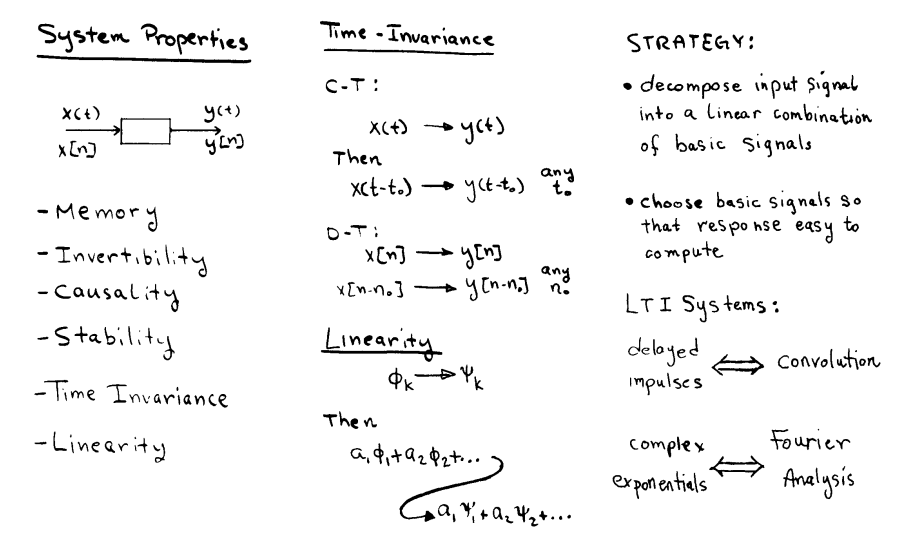
\includegraphics[width=0.8\linewidth]{gambar/03.konvolusi/mk.4.01}
	\end{center}
\end{frame}

\begin{frame}{Superposisi sinyal waktu diskrit}
	\begin{center}
		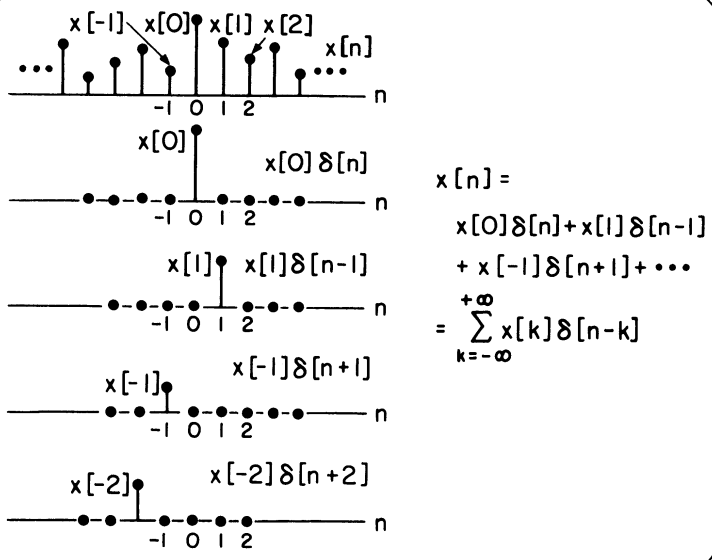
\includegraphics[height=0.8\textheight]{gambar/03.konvolusi/fig.4.01}
	\end{center}
\end{frame}

\begin{frame}{Konvolusi penjumlahan sistem LTI waktu diskrit}
	\begin{center}
		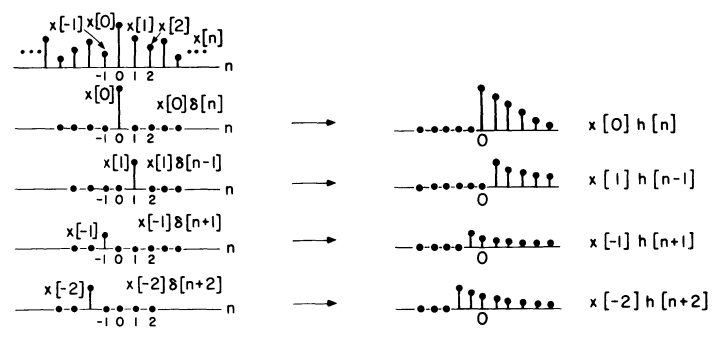
\includegraphics[width=\linewidth]{gambar/03.konvolusi/fig.4.02}
	\end{center}
\end{frame}

\begin{frame}{Konvolusi penjumlahan sistem LTI waktu diskrit}
	\begin{center}
		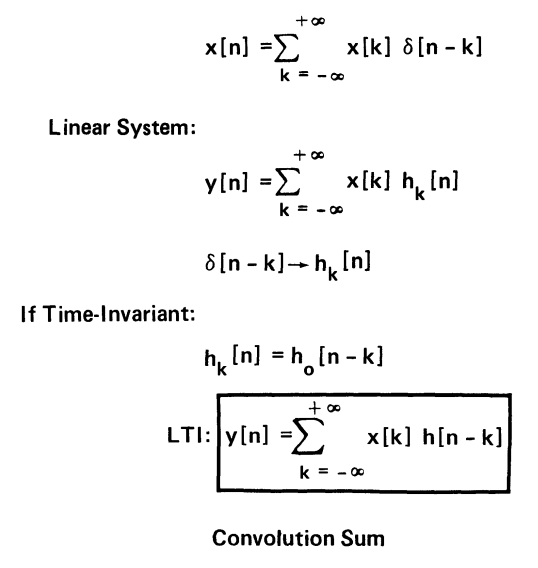
\includegraphics[height=0.8\textheight]{gambar/03.konvolusi/fig.4.03}
	\end{center}
\end{frame}

\begin{frame}{Sinyal waktu kontinu dari kombinasi rectangular pulse}
	\begin{center}
		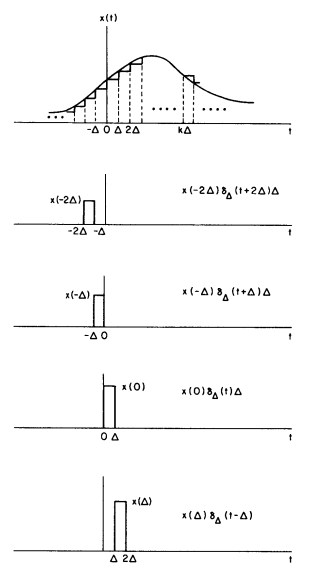
\includegraphics[height=0.8\textheight]{gambar/03.konvolusi/fig.4.04}
	\end{center}
\end{frame}

\begin{frame}{Sinyal waktu kontinu dari kombinasi rectangular pulse}
	\begin{center}
		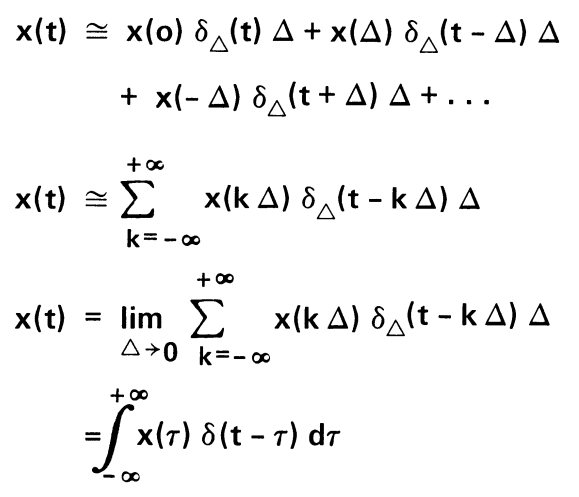
\includegraphics[height=0.8\textheight]{gambar/03.konvolusi/fig.4.05}
	\end{center}
\end{frame}

\begin{frame}{Penurunan konvolusi integral}
	\begin{center}
		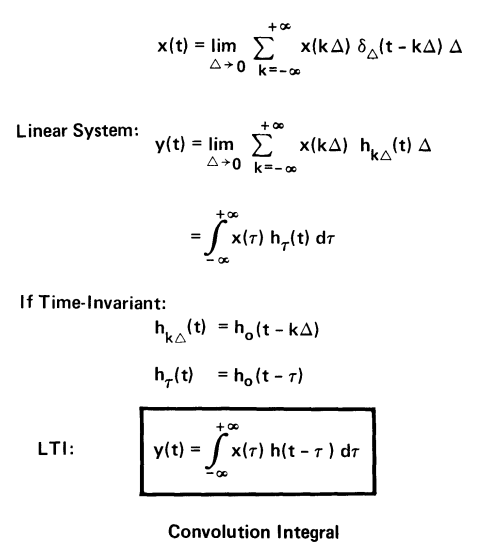
\includegraphics[height=0.8\textheight]{gambar/03.konvolusi/fig.4.06}
	\end{center}
\end{frame}

\begin{frame}{Interpretasi konvolusi integral}
	\begin{center}
		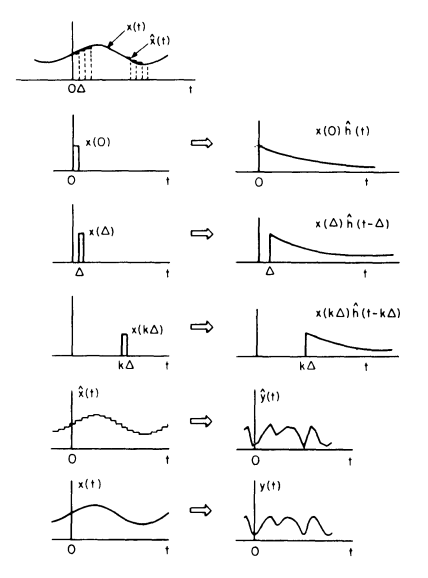
\includegraphics[height=0.8\textheight]{gambar/03.konvolusi/fig.4.07}
	\end{center}
\end{frame}

\begin{frame}{Perbandingan konvolusi penjumlahan dan integral}
	\begin{center}
		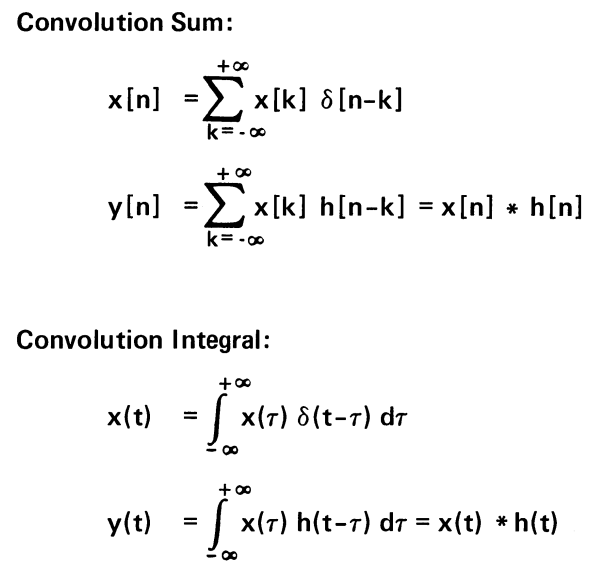
\includegraphics[height=0.8\textheight]{gambar/03.konvolusi/fig.4.08}
	\end{center}
\end{frame}

\begin{frame}{Evaluasi konvolusi penjumlahan}
	\begin{center}
		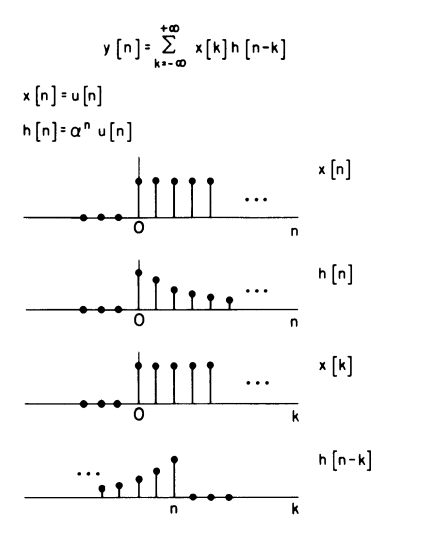
\includegraphics[height=0.8\textheight]{gambar/03.konvolusi/fig.4.09}
	\end{center}
\end{frame}

\begin{frame}{Evaluasi konvolusi integral}
	\begin{center}
		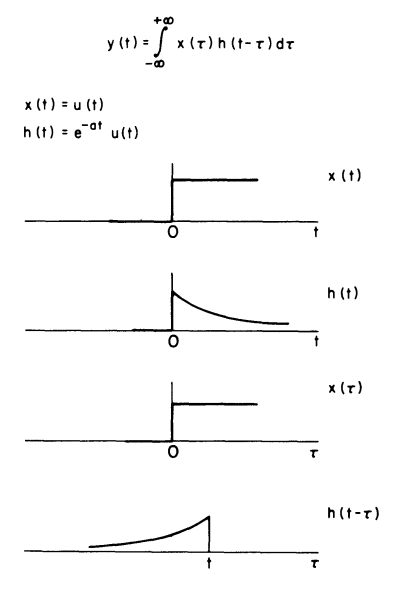
\includegraphics[height=0.8\textheight]{gambar/03.konvolusi/fig.4.10}
	\end{center}
\end{frame}

\begin{frame}{Evaluasi konvolusi integral}
	\begin{center}
		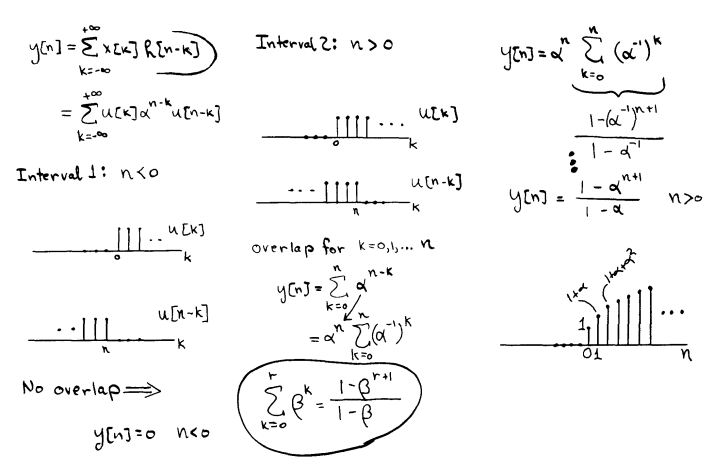
\includegraphics[height=0.8\textheight]{gambar/03.konvolusi/mk.4.02}
	\end{center}
\end{frame}

\begin{frame}{Evaluasi konvolusi integral}
	\begin{center}
		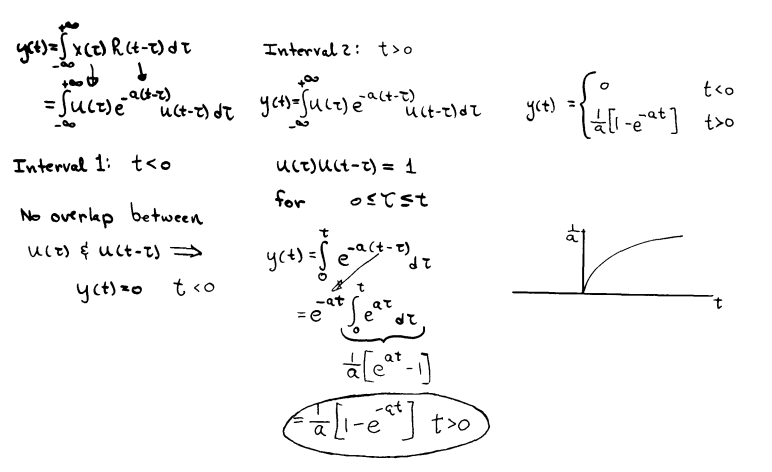
\includegraphics[height=0.8\textheight]{gambar/03.konvolusi/mk.4.03}
	\end{center}
\end{frame}

\end{document}

